\documentclass[tikz,border=8pt]{standalone}
\usepackage{pgfplots}
\usepgfplotslibrary{groupplots}
\pgfplotsset{compat=1.18}
\begin{document}
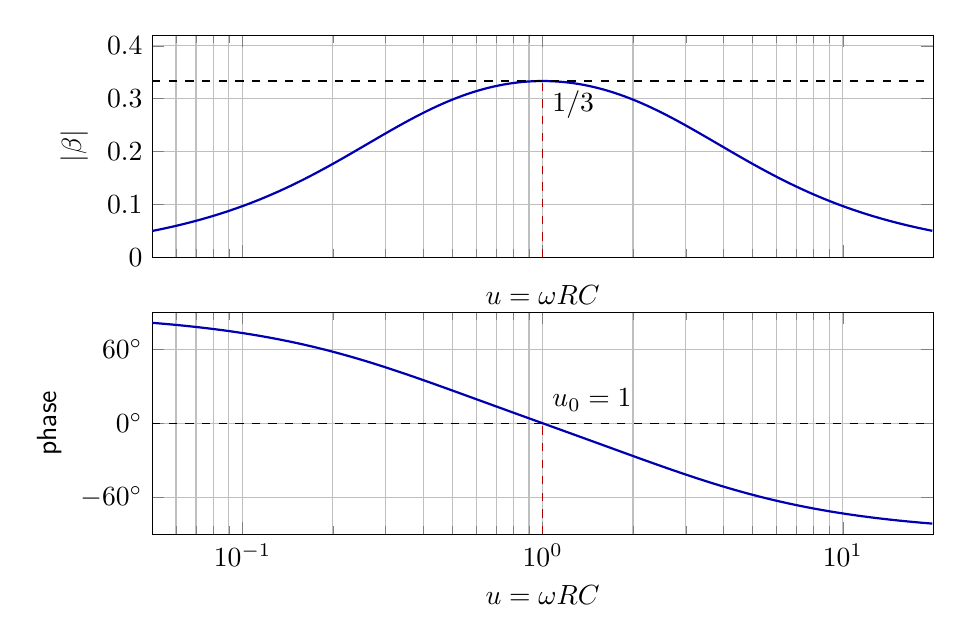
\begin{tikzpicture}[font=\sffamily]
\begin{groupplot}[group style={group size=1 by 2,vertical sep=7mm},width=11.5cm,height=4.4cm,xmode=log,xmin=.05,xmax=20,grid=both,xlabel={$u=\omega RC$}]
\nextgroupplot[ylabel={$|\beta|$},ymin=0,ymax=.42,xticklabels=\empty]
\addplot[blue!70!black,thick,domain=.05:20,samples=500] {x/sqrt((1-x^2)^2+9*x^2)};
\addplot[black,dashed] coordinates {(.05,.333333) (20,.333333)};
\draw[red!70!black,dashed] (axis cs:1,0)--(axis cs:1,.333333);
\node[below right] at (axis cs:1,.333333) {$1/3$};
\nextgroupplot[ylabel={phase},ymin=-90,ymax=90,ytick={-60,0,60},yticklabels={$-60^\circ$,$0^\circ$,$60^\circ$}]
\addplot[blue!70!black,thick,domain=.05:20,samples=500] {atan2(x*(1-x^2),3*x^2)};
\addplot[black,dashed] coordinates {(.05,0) (20,0)};
\draw[red!70!black,dashed] (axis cs:1,-90)--(axis cs:1,0);
\node[above right] at (axis cs:1,2) {$u_0=1$};
\end{groupplot}
\end{tikzpicture}
\end{document}
